%%Capítulo 3 trabajo relacionado 
 \chapter{Trabajo Relacionado}
    \label{cha:TrabajoRelacionado}
   
  Durante la revisión de la literatura referida a este estado del arte, se encontró que existe muy poca bibliografía sobre el tema debido a que las empresas manufactureras de las tarjetas gráficas no liberan suficiente información al público en general, ya que sus diseños no están documentados o se describen a alto nivel que no revelan los detalles técnicos cruciales.
\newline

Se realizó un estudio en \cite{TX2-H} con base en la documentación y pruebas de caja negra sobre la arquitectura Pascal. Como caso de estudio utilizaron el sistema NVIDIA Jetson TX2, que es precisamente el que se tuvo disponible al realizar esta tesis.
%\newline

El estudio tiene como objetivo dar las pautas para realizar normas oficiales de seguridad a los sistemas embebidos heterogéneos y así poder certificar su uso en ambientes críticos. 
\newline

Cada GPU contiene un arreglo de Streaming Multiprocesor (SM) dependiendo del modelo o arquitectura, en donde cada SM puede procesar concurrentemente una misma cantidad de threads. Como ya se mencionó anteriormente, las empresas que producen el hardware no revelan mucho sobre las peculiaridades de cómo se realiza el reparto de recursos para ejecutar las peticiones. Únicamente sabemos que la GPU distribuye los blocks pendientes dentro de los SM en grupos de 32 threads, estos grupos son llamados warps. Un warp es una entidad planificable de un SM.
Un block puede ser asignado únicamente a un SM si este tiene suficientes recursos para recibirlo, si no, esperará hasta que pueda ser lanzado. El cómo realiza esta espera tampoco es revelado por las compañías.
\newline

El sistema Jetson TX2 cuenta con 2 SM, y cada uno con 128 cores que en conjunto pueden procesar concurrentemente 2048 threads\cite{SMJetson}, por lo que cada SM puede manejar un máximo de 64 warps.
\newline

Por ejemplo, en la tabla \ref{tab:asigUnKernelSM} se muestran diversos escenarios en los que se desea agregar kernels para procesar a la tarjeta gráfica.
\newline

  \begin{table}[h!]
      \begin{center}
            \scriptsize
        \begin{tabular}{|m{1.5cm}|m{1cm}|m{1cm}|m{1.5cm}|m{1.5cm}|m{1cm}|m{1cm}|m{1cm}|m{1cm}|m{1.5cm}|}
         \hline
         \cellcolor{lightgray}\textbf{Escenario} &
         \cellcolor{lightgray}\textbf{Kernel} & 
         \cellcolor{lightgray}\textbf{Blocks} &
         \cellcolor{lightgray}\textbf{Threads por block} &
         \cellcolor{lightgray}\textbf{Threads Totales} &
         \cellcolor{lightgray}\textbf{Blocks SM0} &
         \cellcolor{lightgray}\textbf{Warps SM0} &
         \cellcolor{lightgray}\textbf{Blocks SM1} &
         \cellcolor{lightgray}\textbf{Warps SM1} &
         \cellcolor{lightgray}\textbf{Threads utilizados}\\ 
         \hline
         A & K2 & 4 & 512 & 2048 & 4 & 64 & 0 & 0 & 2048\\ 
         \hline
         B & K1 & 16 & 265 & 4096 & 8 & 64 & 8 & 64 & 4096\\ 
         \hline
         C & K3 & 9 & 350 & 3150 & 5 & 55 & 4 & 44 & 3168\\ 
         \hline
           \end{tabular}
        \caption{Asignación de un solo kernel a los SM.}
        \label{tab:asigUnKernelSM}
      \end{center}
    \end{table}
    
    En el escenario \textbf{(A)} (ver figura \ref{fig:asigBlock}) tenemos el kernel \textbf{K2} con 4 blocks y cada uno de 512 threads. La primera condición para poder agregarlo recae en que la totalidad del kernel debe poder ejecutarse en concurrente en la tarjeta gráfica durante un  instante de tiempo. En este caso, recordemos que un SM tiene un máximo de 64 warps disponibles, y el kernel justamente está constituido por esa cantidad, por lo que el planificador de hardware de la tarjeta asigna secuencialmente los blocks a las localidades.
    \newline
    
    En el escenario \textbf{(B)} se agrega un kernel que comprende 16 blocks y cada uno consta de 256 threads por block. En este caso, al lanzarlo se utilizará la totalidad de los recursos de la GPU y los blocks se irán asignando secuencialmente empezando desde la primer localidad del \textbf{SM0} y así sucesivamente hasta que se terminen sus recursos. Cuando esto suceda, se continuará con las primeras localidades de \textbf{SM1} hasta terminar de lanzar todos los blocks del kernel. En caso de que existan recursos para colocar blocks de un kernel al final de \textbf{SM0} pero no los suficientes para colocarlo al inicio de \textbf{SM1}, el kernel no se podrá lanzar, y el planificador por hardware saltará la tarea y asignará otra que ocupe menos recursos.
    \newline
    
    \begin{figure}[ht]
      \centering
        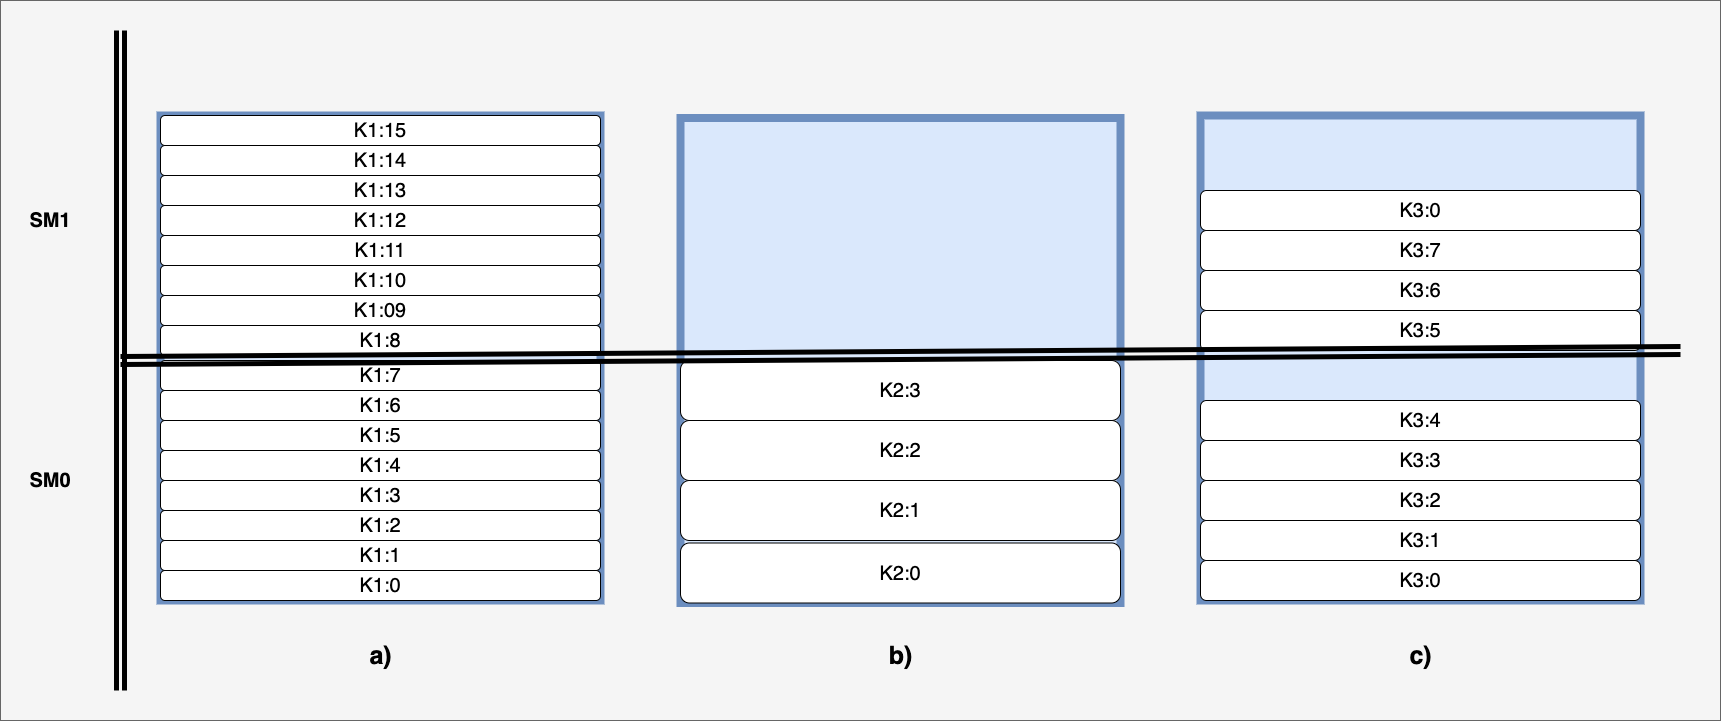
\includegraphics[scale=.275]{asigBlock}
        \caption{Diagrama de asignación de un kernel a los SM.}
        \label{fig:asigBlock}
    \end{figure}
    
    Finalmente, en el escenario \textbf{(C)} deberían ser 54.6 warps en el \textbf{SM0} utilizando 1750 threads, pero en realidad se utilizan 55 warps, con lo que el trabajo de 10 threads y 9 warps se desperdician. En el \textbf{SM1}, deberían ocuparse 43.75 warps, pero se usan 44, dejando 8 threads y 20 warps sin poderse utilizar.
    \newline
    
Habitualmente en sistemas GPGPU se requiere lanzar más de un kernel a la vez, en la tabla \ref{tab:asigVariosKernelsSM} se tienen 3 situaciones en las que esto podría ocurrir.
\newline

    \begin{table}[h!]
      \begin{center}
            \scriptsize
        \begin{tabular}{|m{1.5cm}|m{1cm}|m{1cm}|m{1cm}|m{1cm}|m{1cm}|m{1cm}|m{1cm}|m{1cm}|m{1cm}|m{1cm}|}
         \hline
         \cellcolor{lightgray}\textbf{Escenario} & 
         \cellcolor{lightgray}\textbf{Kernel} & 
         \cellcolor{lightgray}\textbf{Blocks} &
         \cellcolor{lightgray}\textbf{Threads por block} &
         \cellcolor{lightgray}\textbf{Threads por kernel} &
         \cellcolor{lightgray}\textbf{Threads en concurrente} &
         \cellcolor{lightgray}\textbf{Warps} &
         \cellcolor{lightgray}\textbf{Warps aportados a SM0} &
         \cellcolor{lightgray}\textbf{Warps SM0} &
         \cellcolor{lightgray}\textbf{Warps aportados a SM1} &
         \cellcolor{lightgray}\textbf{Warps SM1} \\ 
         \hline
         \multirow{2}{1cm}{D} & K1 & 3  & 512 & 1536 & \multirow{2}{1cm}{4096} & 48 & 48 & \multirow{2}{1cm}{64} & 0  & \multirow{2}{1cm}{64}\\ 
                              & K2 & 10 & 256 & 2560 &                         & 80 & 16 &                       & 64 & \\ 
         \hline \hline
        \multirow{3}{1cm}{E} & K1 & 1 & 1024 & 1024 & \multirow{3}{1cm}{2304} & 32 & 32 & \multirow{3}{1cm}{64} & 0  & \multirow{3}{1cm}{8}\\ 
                             & K2 & 1 & 768  & 768  &                         & 24 & 24 &                      & 0 & \\ 
                             & K3 & 2 & 256  & 512  &                         & 16 & 8 &                       & 8 & \\ 
         \hline \hline
        \multirow{3}{1cm}{F} & K1 & 1 & 768  & 768  & \multirow{3}{1cm}{3072} & 24 & 24 & \multirow{3}{1cm}{24} & 0  & \multirow{3}{1cm}{48}\\ 
                             & K2 & 1 & 1536 & 1536 &                         & 48 & 0  &                       & 48 & \\ 
                             & K3 & 1 & 768  & 768  &                         & 24 & 0  &                       & 0 & \\ 
         \hline
           \end{tabular}
        \caption{Asignación de varios kernels a los SM.}
        \label{tab:asigVariosKernelsSM}
      \end{center}
    \end{table}
    
    En el escenario \textbf{(D)} (ver figura \ref{fig:KernelSM}) se desea asignar dos kernels, uno de 3 blocks y otro de 10. Recordemos que la restricción es que un kernel sólo puede ser asignado si existen suficientes recursos para warps en secuencia. La primer tarea utiliza 48 warps, y la segunda 80, por lo que en \textbf{SM0} podemos asignar los 48 warps del primer kernel más 16 del segundo, y en el \textbf{SM1} colocamos los 64 restantes, ocupando así la totalidad de localidades de la GPU.
    \newline
    
    Continuando con el caso \textbf{(E)}, ahora tenemos 3 kernels, dos de un block con 1024 threads y otro con 768, respectivamente y uno con 2 blocks de 256 threads, en conjunto ocupan 72 warps en total, por lo que podemos asignar los 32 warps del \textbf{K1} al \textbf{SM0}, justo después los 24 del \textbf{K2} y aún sobran 8 warps que sirven perfectamente para ejecutar la mitad de warps del \textbf{K3} y, como las localidades del inicio de \textbf{SM1} están disponibles, se sigue con la asignación de los 8 restantes.
    \newline
    
    El escenario \textbf{(F)} presenta un caso en que se tienen 3 kernels que en conjunto representan 3072 threads, lo que nos hace pensar que muy bien pueden ser ejecutados en concurrente dentro de la GPU, pero el orden de lanzamiento influye de primera mano en la repartición de los recursos. Primero se lanza el kernel \textbf{K1} que constituye 24 warps, después se recibe la petición de  \textbf{K2} con 48, pero como no es posible asignarlo en el \textbf{SM0}, se le asignan las localidades de \textbf{SM1}. Finalmente, desea despachar a \textbf{K3} con 24 warps, pero como la asignación de recursos se realiza de forma secuencial, se empieza a preguntar justo en la siguiente localidad de la última asignada, con lo que ya no es posible lanzar esa tarea, y se deberá esperar a que terminen su ejecución las tareas actuales. Aunque en el \textbf{SM0} sobran recursos que bien podrían aprovecharse, la documentación actual no permite realizarlo, por ello se recurrió a una solución en la sección \ref{secc:balanceador}.
    \newline
    
    \begin{figure}[ht]
      \centering
        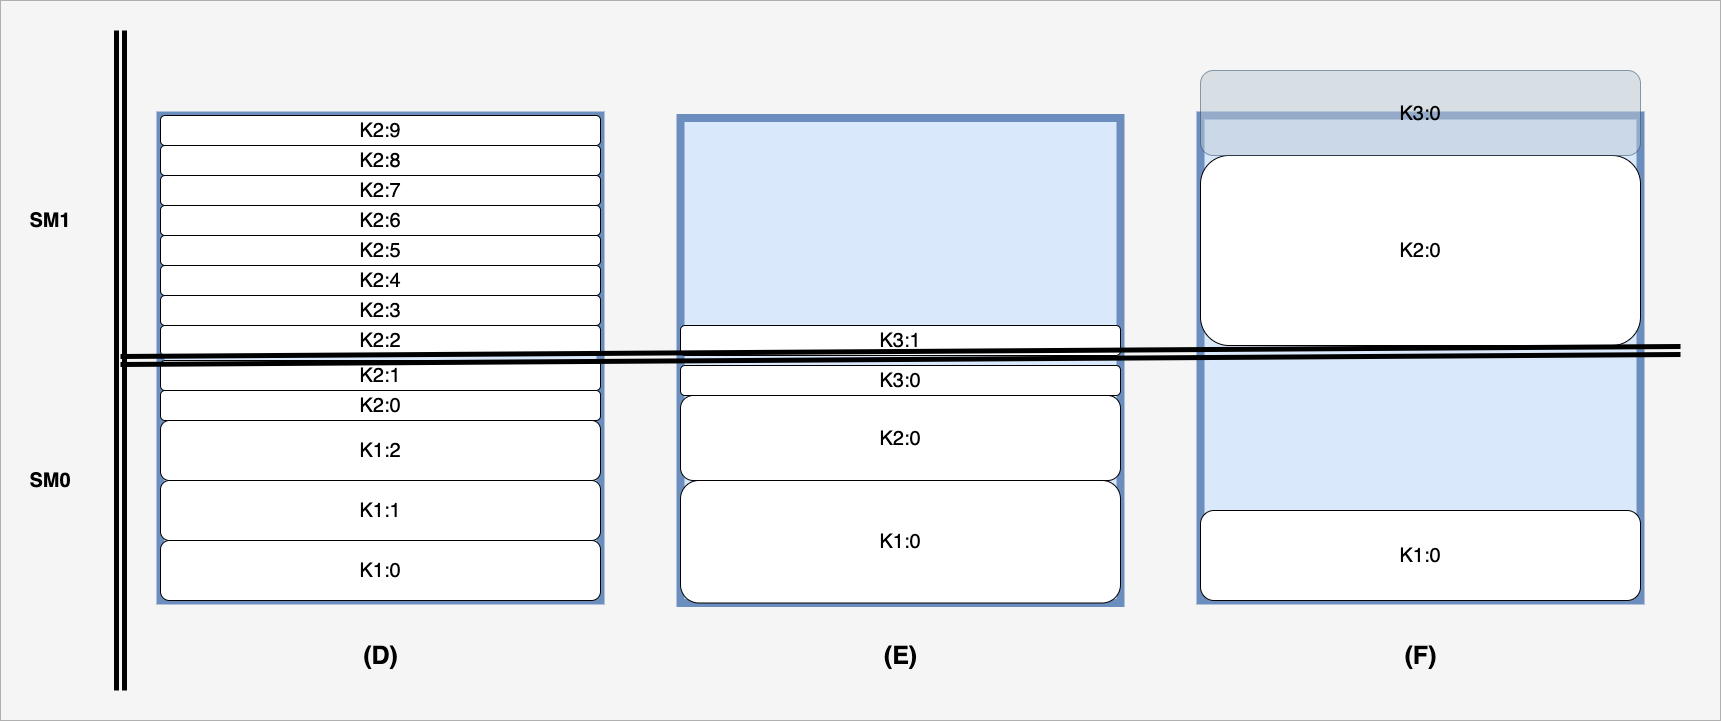
\includegraphics[scale=.275]{KernelSM}
        \caption{Diagrama de asignación de varios kernels a los SM.}
        \label{fig:KernelSM}
    \end{figure}

   Ahora bien, teniendo una referencia por medio de pruebas de software, se puede conocer un poco sobre el funcionamiento de la asignación de kernel a la tarjeta gráfica. Se puede afirmar que es posible gestionar las peticiones de recursos a la GPU, y el programador debe cuidar que tamaño de los bloques de threads sean múltiplos de 32 o al menos potencia de 2 para optimizar los recursos de la tarjeta gráfica y así ejecutar la mayor cantidad posible de tareas concurrentemente.
\newline
    
%Clasificación
Para poder utilizar varias aplicaciones con sistemas en tiempo real complejos es necesario utilizar técnicas de implementación preemptive\cite{RGEM}. Algunos trabajos han utilizado estas técnicas para mejorar el rendimiento de las aplicaciones gráficas en tiempo real, principalmente para la reconstrucción de imágenes en 3D y la detección de rostros\cite{DynSche}.
\newline

La clasificación de la planificación de tareas preemptive esta compuesta de diversos tipos dependiendo de sus técnicas de implementación, cómo se describe en la sección \ref{claspree}. 
%Basado en hardware
Las soluciones basadas en hardware son costosas, ya que debemos desarrollar y construir un dispositivo que auxilie con el cambio de contexto. Por ejemplo, en el artículo \cite{18} se utilizan extensiones de hardware a modo de registros que almacenan el contexto y, en general, las direcciones de memoria que contienen la información necesaria para la restauración de la ejecución de un kernel. 

\vspace{0.3cm}

Se ha propuesto\cite{20} la utilización de extensiones de hardware mediante el intercambio equitativo de recursos entre los núcleos de procesamiento, realizando un cambio de contexto al aplicar el modo preemptive en el espacio de procesamiento. En lugar de intercambiar el contexto de todo el grid, se pretende intercambiar suficientes TB de un kernel en ejecución para que haya suficientes recursos disponibles para despachar la nueva tarea. 

\vspace{0.3cm}

Otra solución la observamos en \cite{8}, donde se desarrolló un compilador que emplea una extensión de hardware para reducir la latencia al implementar el modo preemptive. El compilador inserta puntos preemptive utilizando un análisis del ciclo de vida de los registros. Se utiliza una lógica de compresión-descompresión para disminuir el tamaño del contexto de una tarea. Es decir, cuando el valor almacenado en un determinado registro es siempre igual a lo largo de la ejecución de los TB de un kernel, sólo se guardará un valor durante el cambio de contexto.
\newline
%Para aquellas basadas en software, 

%tenemos por una parte las que parten el kernel como
%Basado en Software : Partición de kernel
El articulo \cite{GPES} implementa \textit{GPES}, una serie de funciones para realizar particiones de kernel y de datos, esto realizando subkernels y dividiendo las transacciones de datos en fragmentos. 
Específicamente, se presenta una técnica de reescritura binaria para reconfigurar de manera transparente el código de los kernel. Mientras que para los kernel un poco más complejos, se desarrolló una técnica de transformación fuente a fuente que compila el código del kernel transformado en binarios CUDA. La prioridad de las tareas esta dada por colas de ejecución. GPES modifica el API de CUDA utilizando las bibliotecas de  \textit{openCUDA} para reconfigurar el código binario de los kernels, esto lo realiza obteniendo un máximo de blocks que se pueden ejecutar por quantum. Para llevarlo a cabo se realiza una transformación fuente a fuente apoyándose en la partición de la transferencia de datos.
\newline

En el artículo \cite{RTFG} se propone un framework de planificación que parte los kernels de la GPU y genera secuencias de lanzamiento en subkernels dinámicamente para entrar en el modo preemptive con la implementación de un divisor de carga de trabajo y de un planificador de tareas. 
Utiliza un divisor de carga de trabajo que fracciona el kernel GPU en múltiples subkernels en tiempo de ejecución para implementar el modo preemptive. Dependiendo del estado actual del sistema y de la prioridad, el divisor de carga de trabajo decide el número y el tamaño de cada subkernel. 

También cuenta con un generador de ejecución planificada, el cual, dependiendo del estado actual de uso de los recursos del sistema y del plazo límite de la tarea, lanza una secuencia de tareas para maximizar el número de aplicaciones cercanas a su plazo vencido.	
\newline

El trabajo \cite{Effisha} describe el framework EffiSha que se basa en un entorno de scripts que permite convertir los kernels automáticamente a modo preemptive. Esta solución consta de componentes que funcionan tanto en tiempo de compilación como en el de ejecución. 
En tiempo de compilación realiza una transformación de fuente a fuente que transforma un programa para la gestión y planificación oportuna de su tiempo de ejecución.
En el código del CPU, reemplaza las llamadas a función de la GPU con las del API de EffiSha, así modifica los kernel GPU para que puedan acelerar el cambio o drenado de contexto durante el tiempo de ejecución. También se analizan e identifican aquellos datos que no se volverán a utilizar después de la restauración de contexto, con lo que ahorra el tiempo de las transacciones de memoria innecesarias.
%\newline

La fase de ejecución consiste en un daemon en el lado del CPU y un proxy de éste en el lado de la GPU. Dicho daemon gestiona el momento en que los kernel deben comenzar, reanudarse o detenerse en la GPU, y dependiendo de la acción se notifica al proceso del CPU que fue lanzado.
%\newline

Como muestran los resultados del trabajo, esta solución funciona bien para kernels con ejecución pequeña porque al tener en el sistema aquellos que salen de la media, la granularidad del TB limita el retraso mínimo preemptive que se puede lograr, resultando muy seguramente en plazos vencidos.
%\newline
 
 Es importante mencionar que el artículo \cite{RGEM} es el primer trabajo que genera un framework para utilizar tareas en tiempo real en tarjetas gráficas. 
 Este trabajo entra dentro de la categoría de colas masivas en paralelo, ya que se basa en la partición en fragmentos de memoria a procesar y cada fragmento es agregado a una cola de procesamiento para ser ejecutado. Su solución es dividir las transacciones de copiado de memoria en varios fragmentos para insertar puntos preemptive. 
 Esto también garantiza que sólo las tareas de mayor prioridad se ejecuten en la GPU en cualquier momento, y así evitar interferencias de rendimiento causadas por lanzamientos concurrentes.

	La primera característica de este framework es que se basa en transacciones de datos preemptive, por lo que los tiempos de bloqueo están limitados para copiar cada fragmento de dato. La segunda característica es que permite lanzar los kernels de diferentes tareas una por una basadas en su prioridad, lo que evita que las tareas con alta prioridad sean interferidas por la carga simultánea de trabajo una vez iniciadas. 
	Sin embargo el lanzamiento del kernel puede bloquearse al haber un kernel de menor prioridad lanzado anteriormente, esto debido al probable alto uso de memoria global.
\newline

El artículo \cite{PreeK} se basa en preguntar continuamente si ha terminado el quantum de una tarea, en caso afirmativo detiene la ejecución e ingresa la siguiente. Las tareas son almacenadas en una cola, por lo que todas tienen la misma prioridad durante la vida del sistema. Se propone un esquema de puntos de control donde se almacena el estado de un kernel en ejecución en la memoria del CPU en vez de la GPU. Para ello, se apoya de una estructura donde se almacena el contexto completo de la tarea. 
Para disminuir la latencia entre cada punto preemptive, se le avisa al framework que se debe tener preparada la estructura de seguridad con directivas \textit{pragma}, antes y después de la ejecución parcial de un kernel. Para ello fue necesario implementar un analizador sintáctico que ayudara al compilador a verificar las modificaciones del código.
\newline

El artículo \cite{IntraNode} propone la creación del framework schedGPU, el cual utiliza el administrador de trabajo Slurm para planificar las tareas. Este framework administra las múltiples solicitudes para acceder a la GPU de forma segura al garantizar que no se produzcan sobrecargas de memoria durante su ejecución. 
Este acceso es controlado mediante bloqueos de archivos, señales del sistema y exclusión mutua.
\newline

SchedGPU utiliza el patrón de diseño cliente-servidor ya que toma cada tarea que busca ser lanzada en la GPU como un cliente que está solicitando memoria a un servidor centralizado (en el mismo nodo), el cual permite que se ejecute si hay suficiente memoria; o en caso contrario, la bloquea hasta que se encuentre memoria necesaria para su funcionamiento. 
El servidor crea un nuevo hilo para cada cliente y mantiene una visión global de la memoria utilizada por todos los clientes a través de la biblioteca de administración de NVIDIA (\textit{NVML})\cite{TORQUE}, esto para evitar la creación de un nuevo contexto que consuma memoria.

La tarea es modificada únicamente al llamar  de manera explícita las funciones de la biblioteca del cliente para previamente asignar la memoria requerida al GPU. Esto acarrea una gran desventaja al considerar tareas donde no siempre es posible conocer la memoria requerida total de GPU, ya que la memoria de la GPU se asigna en tiempo de ejecución. 
En el caso en que dos o más tareas se ejecuten al mismo tiempo y ambas aumenten gradualmente, el uso de la memoria de la GPU se puede llegar a utilizar completamente, con lo que podrán requerir más tiempo para completar la ejecución o directamente lanzar un error de desbordamiento de memoria en tiempo de ejecución.
\newline	
	%Al utilizar schedGPU se encontró que el promedio de la aceleración aumenta 10 veces, comparado con no utilizar el framework. Sin embargo, el promedio de utilización de la memoria también incrementó de 5 a 12 veces.
	
	%Administración dinámica de los núcleos de procesamiento.
	El artículo \cite{Pridriven} presenta una técnica para la ejecución en GPUs llamada \textit{"Planificación de recursos compartidos con reserva de presupuesto"} o por sus siglas en inglés \textit{BR-SRS}, la cual limita el número de núcleos de procesamiento de una GPU para una tarea basándose en su prioridad, esto lo realiza modificando las bibliotecas de  \textit{OpenGL-ES}. 
	Así se previene que una tarea que se encuentra en segundo plano retrase a otra que se encuentra en ejecución, también se minimiza la sobrecarga de planificación al invocarse solamente dos veces, en el inicio de la tarea y en su finalización.
%\newline
%Planificación por prioridad

El único trabajo que utiliza algoritmos para la planificación de tareas en tiempo real, hasta el momento de la revisión del estado del arte es GPUart \cite{GPUArt}. 
Permite la implementación preemptive dentro de los TB y cada uno de estos subkernels se pueden planificar bajo las políticas de Earliest Deadline First (EDF) y de aquellos algoritmos que mantengan la prioridad de las tareas fijas.

GPUart se centra en las GPUs integradas, es decir, en las GPU que se colocan en la misma placa que el CPU. Esto porque permiten tener cero copias de memoria, lo que hace que las transferencias entre CPU y GPU sean nulas al compartir físicamente una memoria común. 
Por ello, GPUart no considera la planificación de transferencias de memoria a través del acceso directo a memoria (DMA).
\newline

A continuación se muestra la tabla \ref{tab:clasifTrabajos} con los trabajos relacionados y la clasificación en la que entran dependiendo de las características con que se ejecutan, así como su referencia en el bibliografía.
 	
  \begin{table}[h!]
      \begin{center}
            \footnotesize
        \begin{tabular}{|m{.6cm}|m{6cm}|m{2.7cm}|m{2.6cm}|m{2.6cm}|}
         \hline
        \cellcolor{lightgray}\textbf{Ref.} & \cellcolor{lightgray} \textbf{Artículo} & \cellcolor{lightgray} \textbf{Clasificación por implementación} & \cellcolor{lightgray} \textbf{Clasificación por planificación} & \cellcolor{lightgray} \textbf{Clasificación por Modificación}  \\ 
         \hline
          \textbf{\cite{18}} & \textbf{Enabling preemptive multiprogramming on GPUs} &  Basado en Hardware: Añade registros para almacenar contexto & Colas masivas en paralelo & Modificación del API\\
           \hline
          \textbf{\cite{20}} & \textbf{Simultaneous Multikernel GPU: Multi-tasking throughput processors via fine-grained sharing} &  Basado en Hardware: Selector de núcleos de procesamiento & Administración dinámica de los núcleos de procesamiento & Modificación del API\\
           \hline
           \textbf{\cite{8}} & \textbf{Enabling Efficient Preemption for SIMT Architectures with Lightweight Context Switching} &  Basado en Hardware: Analizador del ciclo de vida de registros & Administración dinámica de memora &Modificación del API\\
           \hline
             \textbf{\cite{GPES}} & \textbf{GPES: A preemptive execution system for gpgpu computing} & Basado en Software: Partición de kernel & Administración dinámica de memora &Modificación del API\\
           \hline
             \textbf{\cite{RTFG}} & \textbf{Run-Time Scheduling Framework for Event-Driven Applications on a GPU-Based Embedded System*} & Basado en Software: Partición en tareas & Administración dinámica de la memoria & Modificación del código fuente\\
            \hline
            \textbf{\cite{Effisha}} & \textbf{Effisha: A software framework for enabling efficient preemptive scheduling of GPU} & Basado en Software: Entorno de scripts & Colas masivas en paralelo & Modificación del API y código fuente\\
            \hline
          \textbf{\cite{RGEM}} & \textbf{RGEM: A Responsive GPGPU Execution Model for Runtime Engines} & Basado en Software: Partición de kernel & Colas masivas en paralelo & Modificación de código fuente\\
           \hline
           \textbf{\cite{PreeK}} & \textbf{Preemption of a CUDA Kernel Function} & Basado en Software: Partición de kernel & Colas masivas en paralelo & Modificación del API\\
            \hline
            \textbf{\cite{IntraNode}} & \textbf{Intra-Node Memory Safe GPU Co-Scheduling} &Basado en Software: Partición de kernel & Administración dinámica de la memoria & Modificación del API\\
            \hline
            \textbf{\cite{Pridriven}} & \textbf{Priority-driven spatial resource sharing scheduling for embedded graphics processing units} & Basado en Software: Partición en tareas &Administración dinámica de los núcleos de procesamiento & Modificación del API\\
            \hline
          \textbf{\cite{GPUArt}} & \textbf{GpuArt: An application-based limited preemptive gpu real-time scheduler for embedded systems*} & Basado en Software: Partición de kernel & Planificación por prioridad & Modificación de código fuente \\
            \hline
          
                \end{tabular}
        \caption{Matriz de clasificación de trabajos relacionados.}
        \label{tab:clasifTrabajos}
      \end{center}
      \begin{tablenotes}
      \small
      \item \textit{* Artículos que fueron diseñados específicamente para sistemas embebidos.}
    \end{tablenotes}
    \end{table}
    
    
    \begin{comment}
\section{Resumen}
%----------------------------------------------------------------------
    %RESUMEN
Este capítulo presenta los trabajos relacionados con el tema de esta tesis, se analizan 
\begin{itemize}
	\item Planificación de EDF preemptive limitado de sistemas con tareas esporádicas
	 (\textit{Limited Preemption EDF Scheduling of Sporadic Task Systems});
	 %
	 \item Planificación de recursos espaciales compartidos con prioridad para unidades de gráficos embebidos 
	 (\textit{Priority-driven spatial resource sharing scheduling for embedded graphics processing units});
    	 %
	\item Framework para planificación en tiempo de ejecución de aplicaciones con manejo de eventos en sistemas embebidos basados en GPU 
	(\textit{Run-Time Scheduling Framework for Event-Driven Applications on a GPU-Based Embedded System});
		%
	\item Sobre planificación dinámica para la GPU, sus aplicaciones en computación gráfica y más
	(\textit{On Dynamic Scheduling for the GPU and its Applications in Computer Graphics and Beyond}); y
	%
	\item REGM: Un modelo de ejecución GPGPU responsivo para soluciones en tiempo de ejecución
	(\textit{REGM: A Responsive GPGPU Execution Model for Runtime Engines});
	%
    	\item Planificación conjunta con GPU y aseguramiento de la memoria intra-nodo 
	(\textit{Intra-Node Memory Safe GPU Co-Scheduling});
 \end{itemize}
%----------------------------------------------------------------------
\end{comment}
%\vspace{0.3cm}
%Cada sección presenta lo propuesto en el trabajo relacionado, donde se describe el problema, los objetivos y la solución a éste. Brevemente se describe la solución propuesta con los resultados obtenidos y por último se presentan las conclusiones del trabajo.





%The earliest deadline first (EDF) scheduling algorithm is a typical representative of the dynamic priority scheduling algorithm. However, once the system is overloaded, the deadline miss rate increases and the scheduling performance deteriorates sharply, which causes a reduction in system resource utilization.

%En la práctica, ambas visiones de planificación, tanto preemptive, como non-preemptive, tienen ventajas y desventajas comparadas entre sí, por lo que ninguna es superior a la otra. Pero el patrón encontrado es que es necesario en pensar en un Framework qué brinde ayuda a la ejecución de tareas y que permita guardar el contexto en un tiempo específico. 

%Hoy en día, los sistemas embebidos basados en GPU han empezado a considerarse esenciales debido a su alta programabilidad y capacidad de desarrollo con técnicas de alto rendimiento, sumado a su bajo consumo energético. Estos exigen una mayor potencia de cálculo y deben responder a muchos eventos, por lo que se han buscado estrategias, y ahora comparten la memoria entre el CPU y la GPU, lo que resulta en una latencia muy cercana a cero.

%Se han propuesto diversos frameworks de última generación para planificación de tareas para aprovechar el rendimiento de los sistemas embebidos basados en GPU y su bajo consumo de energía.

%%%%%

%En este capítulo se presenta el resumen de tres trabajos relacionados con la evaluación de los patrones de seguridad. El primer trabajo presenta una métrica de seguridad denominada SC la cual contabiliza el total de amenazas mitigadas por patrones de seguridad entre el total de amenazas. Una de las mejoras que propone es utilizar la aproximación \textit{Twin peaks} que produce una nueva arquitectura en cada ciclo contemplando los mismos casos de uso pero a mayor detalle.

%\vspace{0.3cm}

%El segundo trabajo presenta una metodología que consiste en medir qué extensión de una arquitectura está protegida con respecto a las amenazas de seguridad más relevantes. La metodología consiste en cuatro partes: 1) mapeo de las amenazas con los objetivos de seguridad, 2) clasificación de las amenazas de acuerdo a su severidad, 3) determinación de la protección ante una amenaza y 4) cálculo de la cobertura de seguridad. 

%\vspace{0.3cm}

%Por último, el tercer trabajo presenta una metodología que permite elegir los patrones de seguridad con respecto a los objetivos de seguridad y las métricas que evaluarán a los patrones. La metodología se divide en tres fases que son: 1) definición de los patrones de seguridad a partir de los objetivos de seguridad, 2) selección de métricas e 3) interpretación de resultados. Este trabajo tiene como objetivo integrar las métricas a la evaluación de un sistema que está utilizando los patrones de seguridad. 